Dirac and Weyl semimetals are nodal electronic phases of matter in three spatial dimensions. Their low-energy emergent quasiparticle excitations are electronic Dirac~\cite{Dirac28} and Weyl~\cite{Weyl29} fermions. (Contemporary reviews in condensed electronic matter can be found in Ref.~\onlinecite{Ashvin_Weyl_review,TurnerVishwanath13,HasanXuBian15,RMP,Burkov16,JiaXuHasan16,ArmitageMeleVishwanath16,YanFelser17}.) They are three dimensional generalizations of the Dirac fermions that appear in two dimensional graphene~\cite{NetoGuineaPeresNovoselovGeim09} and the surface boundary of a topological insulator~\cite{HasanKane10,QiZhangreview11,HasanMoore11,RMP}. They follow massless quasi-relativistic linear dispersions near nodal points in the energy-momentum space close to the Fermi level. Contrary to accidental degeneracies which can be lifted by generic perturbations, these nodal points are protected by topologies or symmetries. 

A Weyl fermion is {\em chiral} and has a non-trivial winding of a pseudo-spin texture near the singular nodal point in energy-momentum space. This would associate to a non-conservative charge current under a parallel electric and magnetic field and is known as the Adler-Bell-Jackiw anomaly~\cite{Adler69,BellJackiw69}. Thus, in a true three dimensional lattice system, Weyl fermions must come in pairs~\cite{Nielsen_Ninomiya_1981,NielsenNinomiyaPLB1981,NielsenNinomiya83} so that the net chirality, and consequently the anomaly, cancels. Or otherwise, a three dimensional system of a single Weyl fermion must be holographically supported as the boundary of a topological insulator in four dimensions~\cite{ZhangHu01,BernevigChernHuToumbasZhang02,QiHughesZhang08}. On the other hand, a Dirac fermion in three dimensions consists of a pair of Weyl fermions with opposite chiralities. Without symmetries, it is not stable and can turn massive upon inter-Weyl-species coupling. With symmetries, a band crossing can be protected by the distinct symmetry quantum numbers the bands carry along a high symmetry axis. In this article, we focus on the fourfold degenerate Dirac nodal point protected by time-reversal and (screw) rotation symmetry.

In electronic systems, massless Dirac and Weyl fermions appear in gap-closing phase transitions between spin-orbit coupled topological insulators and normal insulators~\cite{Murakami2007}. When inversion or time-reversal symmetry is broken, nodal Weyl points can be separated in energy-momentum space. Such gapless electronic phases are contemporarily referred to as Weyl (semi)metals~\cite{WanVishwanathSavrasovPRB11,YangLuRan11,burkovBalenstPRL11,BurkovBalentsPRB11}. Their boundary surfaces support open Fermi arcs~\cite{WanVishwanathSavrasovPRB11} that connect surface-projected Weyl nodes. Weyl (semi)metals also exhibit exotic transport properties, such as negative magneto-resistance, non-local transport, chiral magnetic effect, and chiral vortical effect~\cite{Burkov_Weyl_electromagnetic_2012,Hosur_Weyl_develop,Lu_anomaly_Weyl_2013,SonSpivak13,Sid_anomaly_Weyl,Marcel_Weyl_response}. There have been numerous first principle calculations~\cite{WengXiZhong16} on proposed materials such as the non-centrosymmetric (La/Lu)Bi$_{1-x}$Sb$_x$Te$_3$~\cite{LiuVanderbilt14}, the TlBiSe$_2$ family~\cite{SinghSharmaLinHasanPrasadBansil12}, the TaAs family~\cite{WengBernevigDai2015,HuangXuZahidTaAs2015}, trigonal Se/Te~\cite{HirayamaOkugawaIshibashiMurakamiMiyake15} and the HgTe class~\cite{RuanXing16}, as well as the time-reversal breaking pyrochlore iridates \cite{WanVishwanathSavrasovPRB11,witczak_kim_weyl_2012,chen_hermele_weyl}, magnetically doped topological and trivial insulator multilayers \cite{burkovBalenstPRL11}, HgCr$_2$Se$_4$~\cite{XuWengWangDaiFang11} and Hg$_{1-x-y}$Cd$_x$Mn$_y$Te~\cite{BulmashLiuQi14}. At the same time, there have also been abundant experimental observations in bulk and surface energy spectra~\cite{HasanXuBelopolskiHuang17} as well as transport~\cite{WangLinWangYuLiao17}. Angle-resolved photoemission spectroscopy (\hypertarget{ARPES}{ARPES}) showed bulk Weyl spectra and surface Fermi arcs in TaAs~\cite{Xu_Weyl_2015_first,Weyl_discovery_TaAs,YangLiuChenTaAs2015,TaAs_Weyl_obeservationDing,BelopolskiZahid16} as well as similar materials such as NbAs, NbP and TaP~\cite{XuNbAs15,LiuChen16}. Other materials such as Ag$_3$BO$_3$, TlTe$_2$O$_6$ and Ag$_2$Se~\cite{ChangHasan16} were observed to host pinned Weyl nodes at high symmetry points. %theory pinned along screw axis {TsirkinSouzaVanderbilt17}
Negative magneto-resistance was reported in TaAs~\cite{Huang_Weyl_2015,Zhang_anomaly_Weyl_2015} as a suggestive signature of the Adler-Bell-Jackiw anomaly. Similar properties were also observed in TaP~\cite{HuMaoTaP17}, NbP and NbAs~\cite{CorinnaNiemannFelserNbP17,LiXuNbAsNbP17,GoothNielschNbP17}, although not without controversies~\cite{SudeshPatnaikNbP17}. 

Weyl points with opposite chiralities cannot be separated in energy-momentum space when both inversion and time reversal symmetries are present. Massless Dirac fermions appear between gap-closing phase transitions between topological and trivial (crystalline) insulators, such as Bi$_{1-x}$Sb$_x$~\cite{TeoFuKane08} and Pb$_{1-x}$Sn$_x$Te~\cite{Hsieh:2012fk}. Critical Dirac (semi)metals were investigated for example in the tunable TlBiSe$_{2-x}$S$_x$~\cite{SatoTakahashi11,SoumaAndo12,XuCavaHasan11}, Bi$_{2−x}$In$_x$Se$_3$~\cite{BrahlekSeongshik12,WuArmitage13} and Hg$_{1-x}$Cd$_x$Te~\cite{OrlitaPotemski14}, as well as the charge balanced BaAgBi~\cite{DuWanXYBi15}, PtBi$_2$, SrSn$_2$As$_2$~\cite{GibsonCava15} and ZrTe$_5$~\cite{LiVallaZrTe516} whose natural states are believed to be close to a topological critical transition. A Dirac (semi)metallic phase can be stablized when the Dirac band crossing is secured along a high symmetry axis and the two crossing bands carry distinct irreducible representations. Theoretical studies include the diamond-structured $\beta$-crystobalite BiO$_2$ family~\cite{BiO3_Dirac_semimetal} No.~227, Fd3m), the orthorhombic body-centered BiZnSiO$_4$ family~\cite{SteinbergYoungZaheerKaneMeleRappe14} (space group No.~74, Imma), the tetragonal Cd$_3$As$_2$~\cite{wangCd3As2PRB13} (space group No.~142, I4$_1$/acd), the hexagonal Na$_3$Bi family~\cite{Dai_predition_Na3Bi}, as well as the filling-enforced non-symmorphic Dirac semimetals~\cite{KonigMermin97,ParameswaranTurnerArovasVishwanath13,WatanabePoVishwanathZaletel15,ChenKimKee16,WatanabePoZaletelVishwanath16} such as the hexagonal TlMo$_3$Te$_3$ family~\cite{GibsonCava15} (space group No.~176, P6$_3$/m), the monoclinic Ca$_2$Pt$_2$Ga (space group No.~15, C2/c), AgF$_2$, Ca$_2$InOsO$_6$ (space group No.~14, P2$_1$/n), and the orthorhombic CsHg$_2$ (space group No.~74, Imma)~\cite{ChenPoNeatonVishwanath16}. At the same time, there are numerous experimental confirmations. They include \ARPES observations on Cd$_2$As$_3$~\cite{Cd3As2Chen2014,neupaneDiracHasan,borisenkoPRLCd3As2}, Na$_3$Bi~\cite{Liu21022014,Xu18122014} and ZrTe$_5$~\cite{LiVallaZrTe516}; scanning tunneling microscopy in Cd$_2$As$_3$~\cite{Yazdani_CdAs}; magneto-transport in Bi$_{1-x}$Sb$_x$~\cite{KimLiBiSb13}, Cd$_2$As$_3$~\cite{liangOngTransportCd3As2,HeLi14,XiangChen15,FengLuCd3As215,LiYuCd3As215,LiWangCd3As216,GuoLeeCd2As316,ZhangXiuCd3As217}, Na$_3$Bi~\cite{Xu18122014,XiongOng15}, ZrTe$_5$~\cite{ZhengMingliangZrTe514,LiVallaZrTe516,LiangOngHallZrTe516,YuanXiuZrTe516}, HfTe$_5$~\cite{WangWangHfTe516} and PtBi$_2$~\cite{GaoTianPtBi217}; magneto-optics~\cite{AkrapOrlitaCd2As316} and anomalous Nernst effect~\cite{LiangOngNernstCd3As217} in Cd$_2$As$_3$, and many more. However, there are also contradicting pieces of evidence, especially in ZrTe$_5$ and HfTe$_5$ that suggest a bulk band gap~\cite{WengDaiFangZrTe514,LiXingZrTe516,WuPanZrTe516,MoreschiniGrioniZrTe516,ManzoniCrepaldiZrTe516,ManzoniParmigianiZrTe517,FanZhouZrTe517}.
%Cd3As2
%SdH\cite{HeLi14,XiangChen15,GuoLeeCd2As316} negative magnetoresistance\cite{liangOngTransportCd3As2} anomalous Nernst effect\cite{LiangOngNernstCd3As217} magneto-optics\cite{AkrapOrlitaCd2As316}
%Na3Bi
%negative magnetoresistance\cite{Xu18122014,XiongOng15}
%ZrTe5
%negative magnetoresistance\cite{ZhengMingliangZrTe514,LiVallaZrTe516} anomalous Hall\cite{LiangOngHallZrTe516}
%HfTe5
%negative magnetoresistance\cite{WangWangHfTe516}
%PtBi2
%magnetoresistance\cite{GaoTianPtBi217}

\begin{figure}[htbp]
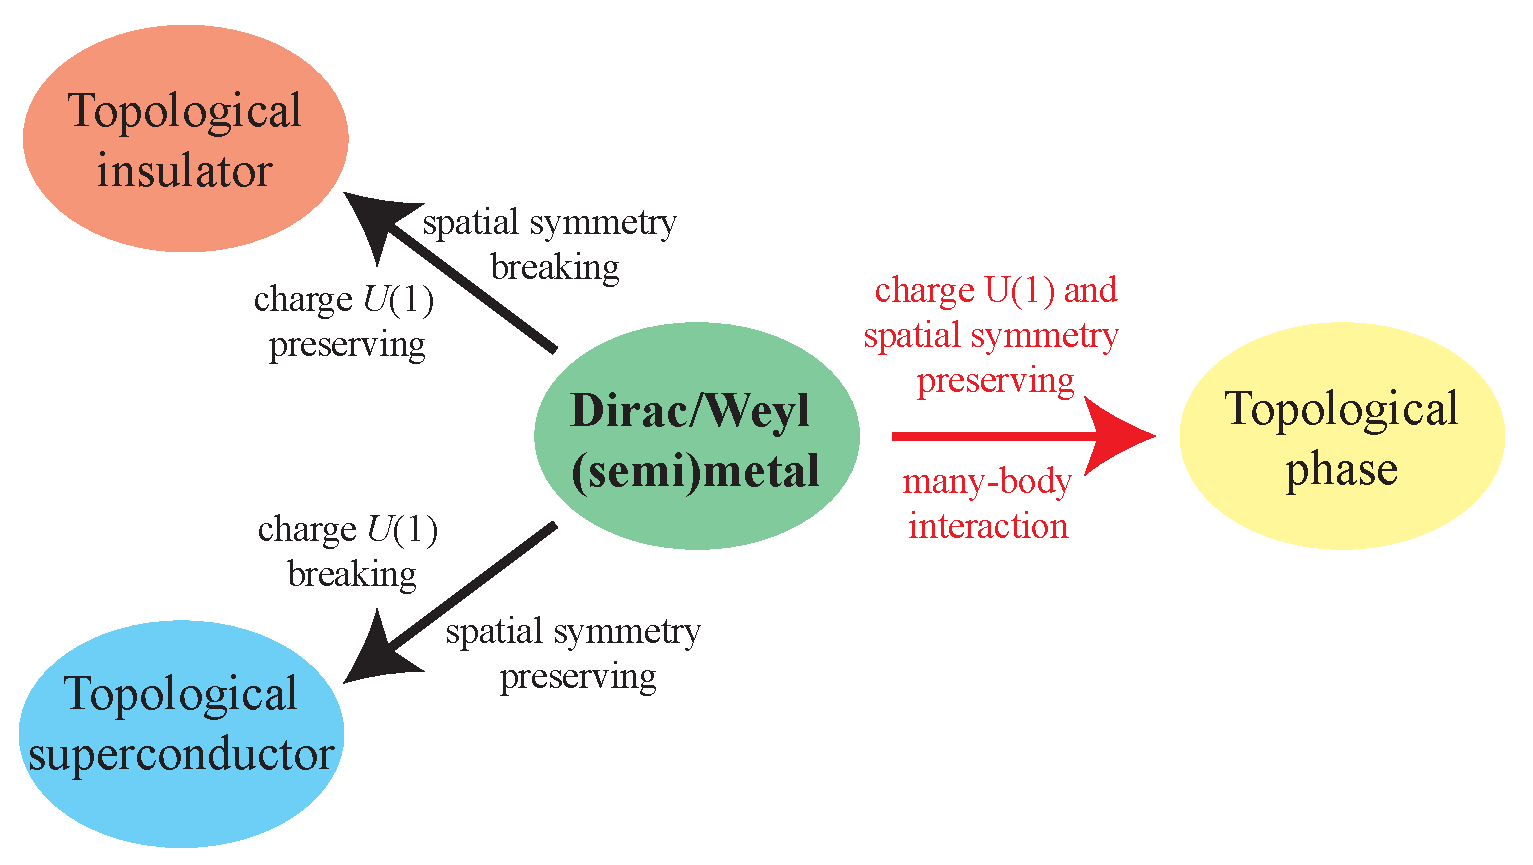
\includegraphics[width=0.45\textwidth]{intro}
\caption{Symmetry breaking single-body gapping versus symmetry preserving many-body gapping of a Dirac/Weyl (semi)metal.}\label{fig:intro}
\end{figure}

Dirac/Weyl (semi)metals are the origins of a wide variety of topological phases in three dimensions (see figure~\ref{fig:intro}). By introducing a spatial or charge $U(1)$ symmetry-breaking single-body mass, they can be turned into a topological insulator or superconductor. The focus of this manuscript is on symmetry-preserving many-body gapping interactions. The resulting insulating topological phase can carry long-range entanglement and a non-trivial topological order. Similar phenomena were theoretically studied on the Dirac surface state of a topological insulator~\cite{WangPotterSenthilgapTI13,MetlitskiKaneFisher13b,ChenFidkowskiVishwanath14,BondersonNayakQi13} and the Majorana surface state of a topological superconductor~\cite{LukaszChenVishwanath,MetlitskiFidkowskiChenVishwanath14}, where symmetry-preserving many-body gapping interactions are possible and lead to non-trivial surface topological orders that support anyonic quasiparticle excitations.

Symmetry-preserving gapping interactions cannot be studied using a single-body mean-field theory. This is because the Dirac/Weyl (semi)metallic phase is protected by symmetries in the single-body setting and any mean-field model with an excitation energy gap must therefore break the symmetry either explicitly or spontaneously. The coupled wire construction can serve as a powerful tool in building an exactly-solvable interacting model and understanding many-body topological phases of this sort. The construction involves a highly anisotropic approximation where the electronic degrees of freedom are confined along an array of continuous one-dimensional wires. Inspired by sliding Luttinger liquids~\cite{OHernLubenskyToner99,EmeryFradkinKivelsonLubensky00,VishwanathCarpentier01,SondhiYang01,MukhopadhyayKaneLubensky01}, the coupled wire construction was pioneered by Kane, Mukhopadhyay and Lubensky~\cite{KaneMukhopadhyayLubensky02} in the study of Laughlin~\cite{Laughlin83} and Haldane-Halperin hierarchy~\cite{Haldane83,Halperin84} fractional quantum Hall states. Later, this theoretical technique was applied in more general fractional quantum Hall states~\cite{TeoKaneCouplewires,KlinovajaLoss14,MengStanoKlinovajaLoss14,SagiOregSternHalperin15,KaneSternHalperin17}, anyon models~\cite{OregSelaStern14,StoudenmireClarkeMongAlicea15}, spin liquids~\cite{MengNeupertGreiterThomale15,GorohovskyPereiraSela15}, (fractional) topological insulators~\cite{NeupertChamonMudryThomale14,KlinovajaTserkovnyak14,SagiOreg14,SagiOreg15,SantosHuangGefenGutman15} and superconductors~\cite{mongg2,SeroussiBergOreg14}, as well as the exploration of symmetries and dualities~\cite{MrossAliceaMotrunich16,MrossAliceaMotrunich17}. Moreover, coupled wire construction has already been used to investigate three dimensional fractional topological phases~\cite{Meng15} and Weyl (semi)metal~\cite{Vazifeh13} even in the strongly-correlated fractional setting~\cite{MengGrushinShtengelBardarson16}.

The microscopic symmetry-preserving many-body interactions in the Dirac surface state on a topological insulator was discussed by Mross, Essin and Alicea in Ref.\onlinecite{MrossEssinAlicea15}. They mimicked the surface Dirac modes using a coupled wire model and proposed explicit symmetric many-body interactions that lead to a variation of gapped and gapless surface states. Motivated by this and also using a coupled wire construction, the microscopic symmetry-preserving many-body gapping of the Majorana topological superconducting surface state was studied by one of us in Ref.\onlinecite{SahooZhangTeo15}. 

In this article, we focus on (i) a coupled wire realization of a Dirac/Weyl (semi)metallic phase protected by antiferromagnetic time-reversal and screw twofold rotation symmetries, (ii) a set of exactly-solvable inter-wire many-body interactions that introduces a finite excitation energy gap while preserving the symmetries, and (iii) an interaction-enabled (semi)metallic electronic phase which is otherwise forbidden by symmetries in the single-body setting.

\subsubsection{Summary of results}\label{sec:introsummary}

We now highlight our results. The first part of this article addresses a mapping between the isotropic massless Dirac fermion in the continuum limit and an anisotropic coupled wire model where the effective low-energy degrees of freedom are confined along a discrete array of 1D continuous wires. We begin with a minimal Dirac (semi)metal equipped with time-reversal and (screw) $\mathcal{C}_2$ rotation symmetries. The mapping to a coupled wire model is achieved by first introducing vortices that break the symmetries microscopically. These vortices are topological line defects that involve spatial winding of symmetry-breaking Dirac mass parameters. Consequently, these vortices host chiral Dirac electronic channels, each of which corresponds to a gapless quasi-1D system where electronic quasiparticles can only propagate in a single direction along the channel and are localized along the perpendiculars. 

When assembled together onto a vortex lattice, the system recovers the screw $\mathcal{C}_2$ rotation symmetry as well as a set of emergent antiferromagnetic symmetries, which are combinations of the broken time-reversal and half-translations. Upon nearest-wire single-body electron backscattering, the electronic band structure disperses linearly and mirrors that of the continuous isotropic Dirac parent state. A symmetry-protected massless Dirac fermion (equivalently a pair of Weyl fermions with opposite chiralities) emerges and captures the low-energy long length scale electronic properties.

This mapping can be qualitatively understood as a coarse-graining procedure where high-energy microscopic electronic degrees of freedom are integrated out. The procedure can be repeated indefinitely and resembles a real-space renormalization. For example, the gapless Dirac electronic structure of the coupled wire model can acquire a finite mass by symmetry-breaking dimerizations. These dimerizations can be arranged in a topological manner that spatially wind non-trivially around a collective vortex. These second-stage vorticies can subsequently be assembled into an array similar to the previous construction except now with a longer lattice constant. The system again recovers a massless Dirac spectrum under inter-vortex electron tunneling in low-energy and long length scale. The mapping therefore establishes an equivalence between the continuous isotropic massless Dirac fermion and the semi-discrete anisotropic coupled Dirac wire model.

The second part of this article addresses non-trivial symmetry-preserving many-body interacting effects beyond the single-body mean-field paradigm. We begin with the anisotropic array of chiral Dirac wires that constitutes a Dirac (semi)metal protected by antiferromagnetic time-reversal (\AFTR) and (screw) $\mathcal{C}_2$ rotation symmetries. We consider an exactly-solvable model of symmetry-preserving inter-wire many-body backscattering interactions. This model is inspired by and can be regarded as a layered version of the symmetric massive interacting surface state of a topological insulator. It is based on a {\em fractionalization} scheme that divides a single chiral Dirac channel into a decoupled pair of identical chiral ``Pfaffian" channels. Each of these fractional channels carries half of the degrees of freedom of the original Dirac wire. For instance, the fractionalization splits the electric and thermal currents exactly in half. %The bipartition is stabilized by many-body interactions and cannot be realized in any single-body mean-field description. 
It leads to the appearance of fractional quasiparticle excitations. For example, a chiral Pfaffian channel also runs along the 1D edge of the particle-hole symmetric Pfaffian fractional quantum Hall state~\cite{Son15,BarkeshliMulliganFisher15,WangSenthil16}, and supports charge $e/4$ Ising and $e/2$ semionic primary fields.

We consider an explicit combination of many-body interwire backscattering interactions that stabilize the fractionalization. Similar coupled wire constructions were applied in the literature to describe topological insulator's surface state~\cite{MrossEssinAlicea15} and $\nu=1/2$ fractional quantum Hall states~\cite{TeoKaneCouplewires,KaneSternHalperin17}. They are higher dimensional analogues of the Affleck-Kennedy-Lieb-Tasaki (AKLT) spin chain model~\cite{AKLT1,AKLT2}. The pair of chiral Pfaffian channels along each wire is backscattered in opposite directions to neighboring wires by the interaction. As a result of this dimerization of fractional degrees of freedom, the model acquires a finite excitation energy gap and at the same time preserves the relevant symmetries.

The coupled wire construction also suggests new {\em interaction-enabled topological (semi)metals}. In the single-body regime, an (antiferromagnetic) time-reversal symmetric Weyl (semi)metal realizable on a three dimensional lattice has a minimum of four momentum-space-separated Weyl nodes. The many-body interacting wire model can be turned into a gapless system where all low-energy degrees of freedom are electronic and are freely described in the single-body non-interacting setting by two and only two separated Weyl nodes. Although the model is antiferromagnetic, we conjecture that similar anomalous Weyl (semi)metal can be enabled by interaction while preserving local time-reversal.

The paper is organized as follows. In section~\ref{sec:DiracSemimetal}, we construct a single-body coupled wire model of a Dirac/Weyl (semi)metal equipped with two emergent antiferromagnetic time-reversal (\AFTR) axes and a (screw) $\mathcal{C}_2$ rotation symmetry. In section~\ref{sec:anomaly}, we establish the equivalence between the isotropic continuum limit and the anisotropic coupled wire limit by a coarse-graining mapping. We also discuss the anomalous aspects of the pair of Weylrmions and different resolutions to the anomaly. Then we describe the gapless surface states of the coupled wire model. \AFTR breaking and preserving surfaces are considered separately in section~\ref{sec:fermiarcAFTRbreaking} and \ref{sec:fermiarcAFTRpreserving} respectively.

In section~\ref{sec:interaction}, we move on to the effect of symmetry-preserving many-body interactions. The fractionalization of a chiral Dirac channel is explained in section~\ref{sec:gluing}, where we review the content of the fractional Pfaffian conformal field theory and establish the decomposition $\mathrm{Dirac}\approx\mathrm{Pfaffian}\otimes\mathrm{Pfaffian}$ through bosonization techniques. The splitting of a Dirac channel is summarized in figure~\ref{fig:fractionalization}. In section~\ref{sec:interactionmodels}, we explicitly construct an exactly-solvable interacting coupled wire model that introduces a finite excitation energy gap to the Dirac system while preserving the relevant symmetries. The many-body interwire backscattering interactions are summarized in figure~\ref{fig:gappinginteraction}. In section~\ref{sec:AFMstablization}, we discuss a plausible stabilization mechanism of the desired interactions through an antiferromagnetic order. In section~\ref{sec:intenable}, we discuss a variation of the model that enables an anomalous topological (semi)metal with two Weyl nodes through interaction. In section~\ref{sec:fracsurface}, we elaborate on the gapless surface states of these new interacting phases.


